\documentclass[landscape]{scrartcl}
\usepackage[top=1.0cm, bottom=1.0cm, left=1cm, right=1cm, marginparwidth=6.0cm, marginparsep=0pt, paperwidth=25.2cm, paperheight=20cm]{geometry}
\usepackage[dvipsnames]{xcolor}
\usepackage{tikz}
\usetikzlibrary{shapes.geometric}
\usepackage{fontspec}
\setmainfont{Tex Gyre Schola}
%\setmainfont[Scale=0.95]{Century Gothic}
\usepackage{contour}
\usepackage{multicol}
\setlength{\columnsep}{1cm}
\usepackage{booktabs}
\usepackage{lipsum}
\usepackage{marginnote}
\usepackage{multirow}
\usepackage{enumitem}
\usepackage{gerrymander}

%\setkomafont{section}{\setmainfont{Tex Gyre Schola}\LARGE\textbf}
\setkomafont{section}{\setmainfont[Scale=0.95]{Century Gothic}\LARGE\bfseries}

% Adjust spacing before and after section headings
\RedeclareSectionCommand[
  runin=false,
  beforeskip=1.0\baselineskip,
  afterskip=0.0\baselineskip
]{section}


\pagestyle{empty}
\begin{document}
{
%\setmainfont[Scale=2.5]{Tex Gyre Schola}
\setmainfont[Scale=3]{Century Gothic}
\begin{center}
\Huge \textbf{Gerrymander}
\end{center}
}

\vfill%\vspace{-0.5cm}

\begin{center}
\scalebox{2.9}{
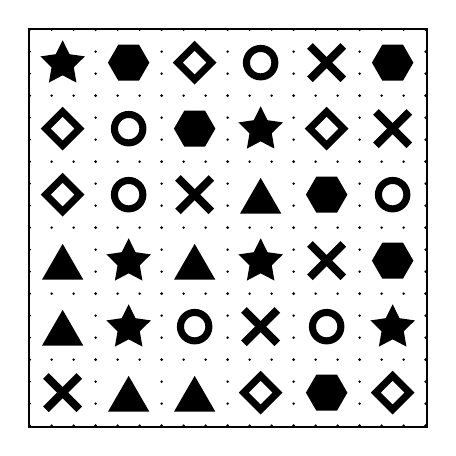
\begin{tikzpicture}
\node[minimum width=0.33in,minimum height=0.33in] at (0.495000in, -0.495000in) {\phantom{.}};
\node[draw=black,circle,inner sep=0.75pt,line width=0.9mm] at (0.495000in, -0.495000in) {\phantom{1}};
\node[minimum width=0.33in,minimum height=0.33in] at (-0.495000in, 0.165000in) {\phantom{.}};
\node[draw=black,circle,inner sep=0.75pt,line width=0.9mm] at (-0.495000in, 0.165000in) {\phantom{1}};
\node[minimum width=0.33in,minimum height=0.33in] at (-0.495000in, 0.495000in) {\phantom{.}};
\node[draw=black,circle,inner sep=0.75pt,line width=0.9mm] at (-0.495000in, 0.495000in) {\phantom{1}};
\node[minimum width=0.33in,minimum height=0.33in] at (-0.165000in, -0.495000in) {\phantom{.}};
\node[draw=black,circle,inner sep=0.75pt,line width=0.9mm] at (-0.165000in, -0.495000in) {\phantom{1}};
\node[minimum width=0.33in,minimum height=0.33in] at (0.165000in, 0.825000in) {\phantom{.}};
\node[draw=black,circle,inner sep=0.75pt,line width=0.9mm] at (0.165000in, 0.825000in) {\phantom{1}};
\node[minimum width=0.33in,minimum height=0.33in] at (0.825000in, 0.165000in) {\phantom{.}};
\node[draw=black,circle,inner sep=0.75pt,line width=0.9mm] at (0.825000in, 0.165000in) {\phantom{1}};
\node[minimum width=0.33in,minimum height=0.33in] at (-0.165000in, 0.165000in) {\phantom{.}};
\node[text=black,rotate=45,inner sep=0pt] at (-0.165000in, 0.165000in) {\rule{6mm}{1mm}};
\node[text=black,rotate=-45,inner sep=0pt] at (-0.165000in, 0.165000in) {\rule{6mm}{1mm}};
\node[minimum width=0.33in,minimum height=0.33in] at (0.495000in, 0.825000in) {\phantom{.}};
\node[text=black,rotate=45,inner sep=0pt] at (0.495000in, 0.825000in) {\rule{6mm}{1mm}};
\node[text=black,rotate=-45,inner sep=0pt] at (0.495000in, 0.825000in) {\rule{6mm}{1mm}};
\node[minimum width=0.33in,minimum height=0.33in] at (0.495000in, -0.165000in) {\phantom{.}};
\node[text=black,rotate=45,inner sep=0pt] at (0.495000in, -0.165000in) {\rule{6mm}{1mm}};
\node[text=black,rotate=-45,inner sep=0pt] at (0.495000in, -0.165000in) {\rule{6mm}{1mm}};
\node[minimum width=0.33in,minimum height=0.33in] at (-0.825000in, -0.825000in) {\phantom{.}};
\node[text=black,rotate=45,inner sep=0pt] at (-0.825000in, -0.825000in) {\rule{6mm}{1mm}};
\node[text=black,rotate=-45,inner sep=0pt] at (-0.825000in, -0.825000in) {\rule{6mm}{1mm}};
\node[minimum width=0.33in,minimum height=0.33in] at (0.165000in, -0.495000in) {\phantom{.}};
\node[text=black,rotate=45,inner sep=0pt] at (0.165000in, -0.495000in) {\rule{6mm}{1mm}};
\node[text=black,rotate=-45,inner sep=0pt] at (0.165000in, -0.495000in) {\rule{6mm}{1mm}};
\node[minimum width=0.33in,minimum height=0.33in] at (0.825000in, 0.495000in) {\phantom{.}};
\node[text=black,rotate=45,inner sep=0pt] at (0.825000in, 0.495000in) {\rule{6mm}{1mm}};
\node[text=black,rotate=-45,inner sep=0pt] at (0.825000in, 0.495000in) {\rule{6mm}{1mm}};
\node[minimum width=0.33in,minimum height=0.33in] at (0.165000in, 0.165000in) {\phantom{.}};
\node[regular polygon,regular polygon sides=3,fill=black,inner sep=1.65pt] at (0.165000in, 0.130000in) {\phantom{.}};
\node[minimum width=0.33in,minimum height=0.33in] at (-0.825000in, -0.495000in) {\phantom{.}};
\node[regular polygon,regular polygon sides=3,fill=black,inner sep=1.65pt] at (-0.825000in, -0.530000in) {\phantom{.}};
\node[minimum width=0.33in,minimum height=0.33in] at (-0.825000in, -0.165000in) {\phantom{.}};
\node[regular polygon,regular polygon sides=3,fill=black,inner sep=1.65pt] at (-0.825000in, -0.200000in) {\phantom{.}};
\node[minimum width=0.33in,minimum height=0.33in] at (-0.165000in, -0.825000in) {\phantom{.}};
\node[regular polygon,regular polygon sides=3,fill=black,inner sep=1.65pt] at (-0.165000in, -0.860000in) {\phantom{.}};
\node[minimum width=0.33in,minimum height=0.33in] at (-0.165000in, -0.165000in) {\phantom{.}};
\node[regular polygon,regular polygon sides=3,fill=black,inner sep=1.65pt] at (-0.165000in, -0.200000in) {\phantom{.}};
\node[minimum width=0.33in,minimum height=0.33in] at (-0.495000in, -0.825000in) {\phantom{.}};
\node[regular polygon,regular polygon sides=3,fill=black,inner sep=1.65pt] at (-0.495000in, -0.860000in) {\phantom{.}};
\node[minimum width=0.33in,minimum height=0.33in] at (0.165000in, -0.825000in) {\phantom{.}};
\node[draw=black,diamond,inner sep=2.35pt,line width=0.9mm] at (0.165000in, -0.825000in) {\phantom{.}};
\node[minimum width=0.33in,minimum height=0.33in] at (0.495000in, 0.495000in) {\phantom{.}};
\node[draw=black,diamond,inner sep=2.35pt,line width=0.9mm] at (0.495000in, 0.495000in) {\phantom{.}};
\node[minimum width=0.33in,minimum height=0.33in] at (0.825000in, -0.825000in) {\phantom{.}};
\node[draw=black,diamond,inner sep=2.35pt,line width=0.9mm] at (0.825000in, -0.825000in) {\phantom{.}};
\node[minimum width=0.33in,minimum height=0.33in] at (-0.825000in, 0.165000in) {\phantom{.}};
\node[draw=black,diamond,inner sep=2.35pt,line width=0.9mm] at (-0.825000in, 0.165000in) {\phantom{.}};
\node[minimum width=0.33in,minimum height=0.33in] at (-0.825000in, 0.495000in) {\phantom{.}};
\node[draw=black,diamond,inner sep=2.35pt,line width=0.9mm] at (-0.825000in, 0.495000in) {\phantom{.}};
\node[minimum width=0.33in,minimum height=0.33in] at (-0.165000in, 0.825000in) {\phantom{.}};
\node[draw=black,diamond,inner sep=2.35pt,line width=0.9mm] at (-0.165000in, 0.825000in) {\phantom{.}};
\node[minimum width=0.33in,minimum height=0.33in] at (-0.825000in, 0.825000in) {\phantom{.}};
\node[star,star points=5,star point ratio=2,fill=black,inner sep=1.6pt] at (-0.825000in, 0.820000in) {\phantom{.}};
\node[minimum width=0.33in,minimum height=0.33in] at (-0.495000in, -0.165000in) {\phantom{.}};
\node[star,star points=5,star point ratio=2,fill=black,inner sep=1.6pt] at (-0.495000in, -0.170000in) {\phantom{.}};
\node[minimum width=0.33in,minimum height=0.33in] at (0.165000in, 0.495000in) {\phantom{.}};
\node[star,star points=5,star point ratio=2,fill=black,inner sep=1.6pt] at (0.165000in, 0.490000in) {\phantom{.}};
\node[minimum width=0.33in,minimum height=0.33in] at (0.165000in, -0.165000in) {\phantom{.}};
\node[star,star points=5,star point ratio=2,fill=black,inner sep=1.6pt] at (0.165000in, -0.170000in) {\phantom{.}};
\node[minimum width=0.33in,minimum height=0.33in] at (-0.495000in, -0.495000in) {\phantom{.}};
\node[star,star points=5,star point ratio=2,fill=black,inner sep=1.6pt] at (-0.495000in, -0.500000in) {\phantom{.}};
\node[minimum width=0.33in,minimum height=0.33in] at (0.825000in, -0.495000in) {\phantom{.}};
\node[star,star points=5,star point ratio=2,fill=black,inner sep=1.6pt] at (0.825000in, -0.500000in) {\phantom{.}};
\node[minimum width=0.33in,minimum height=0.33in] at (0.495000in, -0.825000in) {\phantom{.}};
\node[regular polygon,regular polygon sides=6,fill=black,inner sep=3.2pt] at (0.495000in, -0.825000in) {\phantom{.}};
\node[minimum width=0.33in,minimum height=0.33in] at (0.825000in, -0.165000in) {\phantom{.}};
\node[regular polygon,regular polygon sides=6,fill=black,inner sep=3.2pt] at (0.825000in, -0.165000in) {\phantom{.}};
\node[minimum width=0.33in,minimum height=0.33in] at (0.495000in, 0.165000in) {\phantom{.}};
\node[regular polygon,regular polygon sides=6,fill=black,inner sep=3.2pt] at (0.495000in, 0.165000in) {\phantom{.}};
\node[minimum width=0.33in,minimum height=0.33in] at (-0.165000in, 0.495000in) {\phantom{.}};
\node[regular polygon,regular polygon sides=6,fill=black,inner sep=3.2pt] at (-0.165000in, 0.495000in) {\phantom{.}};
\node[minimum width=0.33in,minimum height=0.33in] at (-0.495000in, 0.825000in) {\phantom{.}};
\node[regular polygon,regular polygon sides=6,fill=black,inner sep=3.2pt] at (-0.495000in, 0.825000in) {\phantom{.}};
\node[minimum width=0.33in,minimum height=0.33in] at (0.825000in, 0.825000in) {\phantom{.}};
\node[regular polygon,regular polygon sides=6,fill=black,inner sep=3.2pt] at (0.825000in, 0.825000in) {\phantom{.}};
\node[inner sep=0.25pt,fill=black,circle] at (-0.990000in, -0.990000in) {\phantom{}};
\node[inner sep=0.25pt,fill=black,circle] at (-0.990000in, -0.660000in) {\phantom{}};
\node[inner sep=0.25pt,fill=black,circle] at (-0.990000in, -0.330000in) {\phantom{}};
\node[inner sep=0.25pt,fill=black,circle] at (-0.990000in, 0.000000in) {\phantom{}};
\node[inner sep=0.25pt,fill=black,circle] at (-0.990000in, 0.330000in) {\phantom{}};
\node[inner sep=0.25pt,fill=black,circle] at (-0.990000in, 0.660000in) {\phantom{}};
\node[inner sep=0.25pt,fill=black,circle] at (-0.990000in, 0.990000in) {\phantom{}};
\node[inner sep=0.25pt,fill=black,circle] at (-0.880000in, -0.990000in) {\phantom{}};
\node[inner sep=0.25pt,fill=black,circle] at (-0.880000in, -0.660000in) {\phantom{}};
\node[inner sep=0.25pt,fill=black,circle] at (-0.880000in, -0.330000in) {\phantom{}};
\node[inner sep=0.25pt,fill=black,circle] at (-0.880000in, 0.000000in) {\phantom{}};
\node[inner sep=0.25pt,fill=black,circle] at (-0.880000in, 0.330000in) {\phantom{}};
\node[inner sep=0.25pt,fill=black,circle] at (-0.880000in, 0.660000in) {\phantom{}};
\node[inner sep=0.25pt,fill=black,circle] at (-0.880000in, 0.990000in) {\phantom{}};
\node[inner sep=0.25pt,fill=black,circle] at (-0.770000in, -0.990000in) {\phantom{}};
\node[inner sep=0.25pt,fill=black,circle] at (-0.770000in, -0.660000in) {\phantom{}};
\node[inner sep=0.25pt,fill=black,circle] at (-0.770000in, -0.330000in) {\phantom{}};
\node[inner sep=0.25pt,fill=black,circle] at (-0.770000in, 0.000000in) {\phantom{}};
\node[inner sep=0.25pt,fill=black,circle] at (-0.770000in, 0.330000in) {\phantom{}};
\node[inner sep=0.25pt,fill=black,circle] at (-0.770000in, 0.660000in) {\phantom{}};
\node[inner sep=0.25pt,fill=black,circle] at (-0.770000in, 0.990000in) {\phantom{}};
\node[inner sep=0.25pt,fill=black,circle] at (-0.660000in, -0.990000in) {\phantom{}};
\node[inner sep=0.25pt,fill=black,circle] at (-0.660000in, -0.660000in) {\phantom{}};
\node[inner sep=0.25pt,fill=black,circle] at (-0.660000in, -0.330000in) {\phantom{}};
\node[inner sep=0.25pt,fill=black,circle] at (-0.660000in, 0.000000in) {\phantom{}};
\node[inner sep=0.25pt,fill=black,circle] at (-0.660000in, 0.330000in) {\phantom{}};
\node[inner sep=0.25pt,fill=black,circle] at (-0.660000in, 0.660000in) {\phantom{}};
\node[inner sep=0.25pt,fill=black,circle] at (-0.660000in, 0.990000in) {\phantom{}};
\node[inner sep=0.25pt,fill=black,circle] at (-0.550000in, -0.990000in) {\phantom{}};
\node[inner sep=0.25pt,fill=black,circle] at (-0.550000in, -0.660000in) {\phantom{}};
\node[inner sep=0.25pt,fill=black,circle] at (-0.550000in, -0.330000in) {\phantom{}};
\node[inner sep=0.25pt,fill=black,circle] at (-0.550000in, 0.000000in) {\phantom{}};
\node[inner sep=0.25pt,fill=black,circle] at (-0.550000in, 0.330000in) {\phantom{}};
\node[inner sep=0.25pt,fill=black,circle] at (-0.550000in, 0.660000in) {\phantom{}};
\node[inner sep=0.25pt,fill=black,circle] at (-0.550000in, 0.990000in) {\phantom{}};
\node[inner sep=0.25pt,fill=black,circle] at (-0.440000in, -0.990000in) {\phantom{}};
\node[inner sep=0.25pt,fill=black,circle] at (-0.440000in, -0.660000in) {\phantom{}};
\node[inner sep=0.25pt,fill=black,circle] at (-0.440000in, -0.330000in) {\phantom{}};
\node[inner sep=0.25pt,fill=black,circle] at (-0.440000in, 0.000000in) {\phantom{}};
\node[inner sep=0.25pt,fill=black,circle] at (-0.440000in, 0.330000in) {\phantom{}};
\node[inner sep=0.25pt,fill=black,circle] at (-0.440000in, 0.660000in) {\phantom{}};
\node[inner sep=0.25pt,fill=black,circle] at (-0.440000in, 0.990000in) {\phantom{}};
\node[inner sep=0.25pt,fill=black,circle] at (-0.330000in, -0.990000in) {\phantom{}};
\node[inner sep=0.25pt,fill=black,circle] at (-0.330000in, -0.660000in) {\phantom{}};
\node[inner sep=0.25pt,fill=black,circle] at (-0.330000in, -0.330000in) {\phantom{}};
\node[inner sep=0.25pt,fill=black,circle] at (-0.330000in, 0.000000in) {\phantom{}};
\node[inner sep=0.25pt,fill=black,circle] at (-0.330000in, 0.330000in) {\phantom{}};
\node[inner sep=0.25pt,fill=black,circle] at (-0.330000in, 0.660000in) {\phantom{}};
\node[inner sep=0.25pt,fill=black,circle] at (-0.330000in, 0.990000in) {\phantom{}};
\node[inner sep=0.25pt,fill=black,circle] at (-0.220000in, -0.990000in) {\phantom{}};
\node[inner sep=0.25pt,fill=black,circle] at (-0.220000in, -0.660000in) {\phantom{}};
\node[inner sep=0.25pt,fill=black,circle] at (-0.220000in, -0.330000in) {\phantom{}};
\node[inner sep=0.25pt,fill=black,circle] at (-0.220000in, 0.000000in) {\phantom{}};
\node[inner sep=0.25pt,fill=black,circle] at (-0.220000in, 0.330000in) {\phantom{}};
\node[inner sep=0.25pt,fill=black,circle] at (-0.220000in, 0.660000in) {\phantom{}};
\node[inner sep=0.25pt,fill=black,circle] at (-0.220000in, 0.990000in) {\phantom{}};
\node[inner sep=0.25pt,fill=black,circle] at (-0.110000in, -0.990000in) {\phantom{}};
\node[inner sep=0.25pt,fill=black,circle] at (-0.110000in, -0.660000in) {\phantom{}};
\node[inner sep=0.25pt,fill=black,circle] at (-0.110000in, -0.330000in) {\phantom{}};
\node[inner sep=0.25pt,fill=black,circle] at (-0.110000in, 0.000000in) {\phantom{}};
\node[inner sep=0.25pt,fill=black,circle] at (-0.110000in, 0.330000in) {\phantom{}};
\node[inner sep=0.25pt,fill=black,circle] at (-0.110000in, 0.660000in) {\phantom{}};
\node[inner sep=0.25pt,fill=black,circle] at (-0.110000in, 0.990000in) {\phantom{}};
\node[inner sep=0.25pt,fill=black,circle] at (-0.000000in, -0.990000in) {\phantom{}};
\node[inner sep=0.25pt,fill=black,circle] at (-0.000000in, -0.660000in) {\phantom{}};
\node[inner sep=0.25pt,fill=black,circle] at (-0.000000in, -0.330000in) {\phantom{}};
\node[inner sep=0.25pt,fill=black,circle] at (-0.000000in, 0.000000in) {\phantom{}};
\node[inner sep=0.25pt,fill=black,circle] at (-0.000000in, 0.330000in) {\phantom{}};
\node[inner sep=0.25pt,fill=black,circle] at (-0.000000in, 0.660000in) {\phantom{}};
\node[inner sep=0.25pt,fill=black,circle] at (-0.000000in, 0.990000in) {\phantom{}};
\node[inner sep=0.25pt,fill=black,circle] at (0.110000in, -0.990000in) {\phantom{}};
\node[inner sep=0.25pt,fill=black,circle] at (0.110000in, -0.660000in) {\phantom{}};
\node[inner sep=0.25pt,fill=black,circle] at (0.110000in, -0.330000in) {\phantom{}};
\node[inner sep=0.25pt,fill=black,circle] at (0.110000in, 0.000000in) {\phantom{}};
\node[inner sep=0.25pt,fill=black,circle] at (0.110000in, 0.330000in) {\phantom{}};
\node[inner sep=0.25pt,fill=black,circle] at (0.110000in, 0.660000in) {\phantom{}};
\node[inner sep=0.25pt,fill=black,circle] at (0.110000in, 0.990000in) {\phantom{}};
\node[inner sep=0.25pt,fill=black,circle] at (0.220000in, -0.990000in) {\phantom{}};
\node[inner sep=0.25pt,fill=black,circle] at (0.220000in, -0.660000in) {\phantom{}};
\node[inner sep=0.25pt,fill=black,circle] at (0.220000in, -0.330000in) {\phantom{}};
\node[inner sep=0.25pt,fill=black,circle] at (0.220000in, 0.000000in) {\phantom{}};
\node[inner sep=0.25pt,fill=black,circle] at (0.220000in, 0.330000in) {\phantom{}};
\node[inner sep=0.25pt,fill=black,circle] at (0.220000in, 0.660000in) {\phantom{}};
\node[inner sep=0.25pt,fill=black,circle] at (0.220000in, 0.990000in) {\phantom{}};
\node[inner sep=0.25pt,fill=black,circle] at (0.330000in, -0.990000in) {\phantom{}};
\node[inner sep=0.25pt,fill=black,circle] at (0.330000in, -0.660000in) {\phantom{}};
\node[inner sep=0.25pt,fill=black,circle] at (0.330000in, -0.330000in) {\phantom{}};
\node[inner sep=0.25pt,fill=black,circle] at (0.330000in, 0.000000in) {\phantom{}};
\node[inner sep=0.25pt,fill=black,circle] at (0.330000in, 0.330000in) {\phantom{}};
\node[inner sep=0.25pt,fill=black,circle] at (0.330000in, 0.660000in) {\phantom{}};
\node[inner sep=0.25pt,fill=black,circle] at (0.330000in, 0.990000in) {\phantom{}};
\node[inner sep=0.25pt,fill=black,circle] at (0.440000in, -0.990000in) {\phantom{}};
\node[inner sep=0.25pt,fill=black,circle] at (0.440000in, -0.660000in) {\phantom{}};
\node[inner sep=0.25pt,fill=black,circle] at (0.440000in, -0.330000in) {\phantom{}};
\node[inner sep=0.25pt,fill=black,circle] at (0.440000in, 0.000000in) {\phantom{}};
\node[inner sep=0.25pt,fill=black,circle] at (0.440000in, 0.330000in) {\phantom{}};
\node[inner sep=0.25pt,fill=black,circle] at (0.440000in, 0.660000in) {\phantom{}};
\node[inner sep=0.25pt,fill=black,circle] at (0.440000in, 0.990000in) {\phantom{}};
\node[inner sep=0.25pt,fill=black,circle] at (0.550000in, -0.990000in) {\phantom{}};
\node[inner sep=0.25pt,fill=black,circle] at (0.550000in, -0.660000in) {\phantom{}};
\node[inner sep=0.25pt,fill=black,circle] at (0.550000in, -0.330000in) {\phantom{}};
\node[inner sep=0.25pt,fill=black,circle] at (0.550000in, 0.000000in) {\phantom{}};
\node[inner sep=0.25pt,fill=black,circle] at (0.550000in, 0.330000in) {\phantom{}};
\node[inner sep=0.25pt,fill=black,circle] at (0.550000in, 0.660000in) {\phantom{}};
\node[inner sep=0.25pt,fill=black,circle] at (0.550000in, 0.990000in) {\phantom{}};
\node[inner sep=0.25pt,fill=black,circle] at (0.660000in, -0.990000in) {\phantom{}};
\node[inner sep=0.25pt,fill=black,circle] at (0.660000in, -0.660000in) {\phantom{}};
\node[inner sep=0.25pt,fill=black,circle] at (0.660000in, -0.330000in) {\phantom{}};
\node[inner sep=0.25pt,fill=black,circle] at (0.660000in, 0.000000in) {\phantom{}};
\node[inner sep=0.25pt,fill=black,circle] at (0.660000in, 0.330000in) {\phantom{}};
\node[inner sep=0.25pt,fill=black,circle] at (0.660000in, 0.660000in) {\phantom{}};
\node[inner sep=0.25pt,fill=black,circle] at (0.660000in, 0.990000in) {\phantom{}};
\node[inner sep=0.25pt,fill=black,circle] at (0.770000in, -0.990000in) {\phantom{}};
\node[inner sep=0.25pt,fill=black,circle] at (0.770000in, -0.660000in) {\phantom{}};
\node[inner sep=0.25pt,fill=black,circle] at (0.770000in, -0.330000in) {\phantom{}};
\node[inner sep=0.25pt,fill=black,circle] at (0.770000in, 0.000000in) {\phantom{}};
\node[inner sep=0.25pt,fill=black,circle] at (0.770000in, 0.330000in) {\phantom{}};
\node[inner sep=0.25pt,fill=black,circle] at (0.770000in, 0.660000in) {\phantom{}};
\node[inner sep=0.25pt,fill=black,circle] at (0.770000in, 0.990000in) {\phantom{}};
\node[inner sep=0.25pt,fill=black,circle] at (0.880000in, -0.990000in) {\phantom{}};
\node[inner sep=0.25pt,fill=black,circle] at (0.880000in, -0.660000in) {\phantom{}};
\node[inner sep=0.25pt,fill=black,circle] at (0.880000in, -0.330000in) {\phantom{}};
\node[inner sep=0.25pt,fill=black,circle] at (0.880000in, 0.000000in) {\phantom{}};
\node[inner sep=0.25pt,fill=black,circle] at (0.880000in, 0.330000in) {\phantom{}};
\node[inner sep=0.25pt,fill=black,circle] at (0.880000in, 0.660000in) {\phantom{}};
\node[inner sep=0.25pt,fill=black,circle] at (0.880000in, 0.990000in) {\phantom{}};
\node[inner sep=0.25pt,fill=black,circle] at (0.990000in, -0.990000in) {\phantom{}};
\node[inner sep=0.25pt,fill=black,circle] at (0.990000in, -0.660000in) {\phantom{}};
\node[inner sep=0.25pt,fill=black,circle] at (0.990000in, -0.330000in) {\phantom{}};
\node[inner sep=0.25pt,fill=black,circle] at (0.990000in, 0.000000in) {\phantom{}};
\node[inner sep=0.25pt,fill=black,circle] at (0.990000in, 0.330000in) {\phantom{}};
\node[inner sep=0.25pt,fill=black,circle] at (0.990000in, 0.660000in) {\phantom{}};
\node[inner sep=0.25pt,fill=black,circle] at (0.990000in, 0.990000in) {\phantom{}};
\node[inner sep=0.25pt,fill=black,circle] at (-0.990000in, -0.990000in) {\phantom{}};
\node[inner sep=0.25pt,fill=black,circle] at (-0.990000in, -0.880000in) {\phantom{}};
\node[inner sep=0.25pt,fill=black,circle] at (-0.990000in, -0.770000in) {\phantom{}};
\node[inner sep=0.25pt,fill=black,circle] at (-0.990000in, -0.660000in) {\phantom{}};
\node[inner sep=0.25pt,fill=black,circle] at (-0.990000in, -0.550000in) {\phantom{}};
\node[inner sep=0.25pt,fill=black,circle] at (-0.990000in, -0.440000in) {\phantom{}};
\node[inner sep=0.25pt,fill=black,circle] at (-0.990000in, -0.330000in) {\phantom{}};
\node[inner sep=0.25pt,fill=black,circle] at (-0.990000in, -0.220000in) {\phantom{}};
\node[inner sep=0.25pt,fill=black,circle] at (-0.990000in, -0.110000in) {\phantom{}};
\node[inner sep=0.25pt,fill=black,circle] at (-0.990000in, -0.000000in) {\phantom{}};
\node[inner sep=0.25pt,fill=black,circle] at (-0.990000in, 0.110000in) {\phantom{}};
\node[inner sep=0.25pt,fill=black,circle] at (-0.990000in, 0.220000in) {\phantom{}};
\node[inner sep=0.25pt,fill=black,circle] at (-0.990000in, 0.330000in) {\phantom{}};
\node[inner sep=0.25pt,fill=black,circle] at (-0.990000in, 0.440000in) {\phantom{}};
\node[inner sep=0.25pt,fill=black,circle] at (-0.990000in, 0.550000in) {\phantom{}};
\node[inner sep=0.25pt,fill=black,circle] at (-0.990000in, 0.660000in) {\phantom{}};
\node[inner sep=0.25pt,fill=black,circle] at (-0.990000in, 0.770000in) {\phantom{}};
\node[inner sep=0.25pt,fill=black,circle] at (-0.990000in, 0.880000in) {\phantom{}};
\node[inner sep=0.25pt,fill=black,circle] at (-0.990000in, 0.990000in) {\phantom{}};
\node[inner sep=0.25pt,fill=black,circle] at (-0.660000in, -0.990000in) {\phantom{}};
\node[inner sep=0.25pt,fill=black,circle] at (-0.660000in, -0.880000in) {\phantom{}};
\node[inner sep=0.25pt,fill=black,circle] at (-0.660000in, -0.770000in) {\phantom{}};
\node[inner sep=0.25pt,fill=black,circle] at (-0.660000in, -0.660000in) {\phantom{}};
\node[inner sep=0.25pt,fill=black,circle] at (-0.660000in, -0.550000in) {\phantom{}};
\node[inner sep=0.25pt,fill=black,circle] at (-0.660000in, -0.440000in) {\phantom{}};
\node[inner sep=0.25pt,fill=black,circle] at (-0.660000in, -0.330000in) {\phantom{}};
\node[inner sep=0.25pt,fill=black,circle] at (-0.660000in, -0.220000in) {\phantom{}};
\node[inner sep=0.25pt,fill=black,circle] at (-0.660000in, -0.110000in) {\phantom{}};
\node[inner sep=0.25pt,fill=black,circle] at (-0.660000in, -0.000000in) {\phantom{}};
\node[inner sep=0.25pt,fill=black,circle] at (-0.660000in, 0.110000in) {\phantom{}};
\node[inner sep=0.25pt,fill=black,circle] at (-0.660000in, 0.220000in) {\phantom{}};
\node[inner sep=0.25pt,fill=black,circle] at (-0.660000in, 0.330000in) {\phantom{}};
\node[inner sep=0.25pt,fill=black,circle] at (-0.660000in, 0.440000in) {\phantom{}};
\node[inner sep=0.25pt,fill=black,circle] at (-0.660000in, 0.550000in) {\phantom{}};
\node[inner sep=0.25pt,fill=black,circle] at (-0.660000in, 0.660000in) {\phantom{}};
\node[inner sep=0.25pt,fill=black,circle] at (-0.660000in, 0.770000in) {\phantom{}};
\node[inner sep=0.25pt,fill=black,circle] at (-0.660000in, 0.880000in) {\phantom{}};
\node[inner sep=0.25pt,fill=black,circle] at (-0.660000in, 0.990000in) {\phantom{}};
\node[inner sep=0.25pt,fill=black,circle] at (-0.330000in, -0.990000in) {\phantom{}};
\node[inner sep=0.25pt,fill=black,circle] at (-0.330000in, -0.880000in) {\phantom{}};
\node[inner sep=0.25pt,fill=black,circle] at (-0.330000in, -0.770000in) {\phantom{}};
\node[inner sep=0.25pt,fill=black,circle] at (-0.330000in, -0.660000in) {\phantom{}};
\node[inner sep=0.25pt,fill=black,circle] at (-0.330000in, -0.550000in) {\phantom{}};
\node[inner sep=0.25pt,fill=black,circle] at (-0.330000in, -0.440000in) {\phantom{}};
\node[inner sep=0.25pt,fill=black,circle] at (-0.330000in, -0.330000in) {\phantom{}};
\node[inner sep=0.25pt,fill=black,circle] at (-0.330000in, -0.220000in) {\phantom{}};
\node[inner sep=0.25pt,fill=black,circle] at (-0.330000in, -0.110000in) {\phantom{}};
\node[inner sep=0.25pt,fill=black,circle] at (-0.330000in, -0.000000in) {\phantom{}};
\node[inner sep=0.25pt,fill=black,circle] at (-0.330000in, 0.110000in) {\phantom{}};
\node[inner sep=0.25pt,fill=black,circle] at (-0.330000in, 0.220000in) {\phantom{}};
\node[inner sep=0.25pt,fill=black,circle] at (-0.330000in, 0.330000in) {\phantom{}};
\node[inner sep=0.25pt,fill=black,circle] at (-0.330000in, 0.440000in) {\phantom{}};
\node[inner sep=0.25pt,fill=black,circle] at (-0.330000in, 0.550000in) {\phantom{}};
\node[inner sep=0.25pt,fill=black,circle] at (-0.330000in, 0.660000in) {\phantom{}};
\node[inner sep=0.25pt,fill=black,circle] at (-0.330000in, 0.770000in) {\phantom{}};
\node[inner sep=0.25pt,fill=black,circle] at (-0.330000in, 0.880000in) {\phantom{}};
\node[inner sep=0.25pt,fill=black,circle] at (-0.330000in, 0.990000in) {\phantom{}};
\node[inner sep=0.25pt,fill=black,circle] at (0.000000in, -0.990000in) {\phantom{}};
\node[inner sep=0.25pt,fill=black,circle] at (0.000000in, -0.880000in) {\phantom{}};
\node[inner sep=0.25pt,fill=black,circle] at (0.000000in, -0.770000in) {\phantom{}};
\node[inner sep=0.25pt,fill=black,circle] at (0.000000in, -0.660000in) {\phantom{}};
\node[inner sep=0.25pt,fill=black,circle] at (0.000000in, -0.550000in) {\phantom{}};
\node[inner sep=0.25pt,fill=black,circle] at (0.000000in, -0.440000in) {\phantom{}};
\node[inner sep=0.25pt,fill=black,circle] at (0.000000in, -0.330000in) {\phantom{}};
\node[inner sep=0.25pt,fill=black,circle] at (0.000000in, -0.220000in) {\phantom{}};
\node[inner sep=0.25pt,fill=black,circle] at (0.000000in, -0.110000in) {\phantom{}};
\node[inner sep=0.25pt,fill=black,circle] at (0.000000in, -0.000000in) {\phantom{}};
\node[inner sep=0.25pt,fill=black,circle] at (0.000000in, 0.110000in) {\phantom{}};
\node[inner sep=0.25pt,fill=black,circle] at (0.000000in, 0.220000in) {\phantom{}};
\node[inner sep=0.25pt,fill=black,circle] at (0.000000in, 0.330000in) {\phantom{}};
\node[inner sep=0.25pt,fill=black,circle] at (0.000000in, 0.440000in) {\phantom{}};
\node[inner sep=0.25pt,fill=black,circle] at (0.000000in, 0.550000in) {\phantom{}};
\node[inner sep=0.25pt,fill=black,circle] at (0.000000in, 0.660000in) {\phantom{}};
\node[inner sep=0.25pt,fill=black,circle] at (0.000000in, 0.770000in) {\phantom{}};
\node[inner sep=0.25pt,fill=black,circle] at (0.000000in, 0.880000in) {\phantom{}};
\node[inner sep=0.25pt,fill=black,circle] at (0.000000in, 0.990000in) {\phantom{}};
\node[inner sep=0.25pt,fill=black,circle] at (0.330000in, -0.990000in) {\phantom{}};
\node[inner sep=0.25pt,fill=black,circle] at (0.330000in, -0.880000in) {\phantom{}};
\node[inner sep=0.25pt,fill=black,circle] at (0.330000in, -0.770000in) {\phantom{}};
\node[inner sep=0.25pt,fill=black,circle] at (0.330000in, -0.660000in) {\phantom{}};
\node[inner sep=0.25pt,fill=black,circle] at (0.330000in, -0.550000in) {\phantom{}};
\node[inner sep=0.25pt,fill=black,circle] at (0.330000in, -0.440000in) {\phantom{}};
\node[inner sep=0.25pt,fill=black,circle] at (0.330000in, -0.330000in) {\phantom{}};
\node[inner sep=0.25pt,fill=black,circle] at (0.330000in, -0.220000in) {\phantom{}};
\node[inner sep=0.25pt,fill=black,circle] at (0.330000in, -0.110000in) {\phantom{}};
\node[inner sep=0.25pt,fill=black,circle] at (0.330000in, -0.000000in) {\phantom{}};
\node[inner sep=0.25pt,fill=black,circle] at (0.330000in, 0.110000in) {\phantom{}};
\node[inner sep=0.25pt,fill=black,circle] at (0.330000in, 0.220000in) {\phantom{}};
\node[inner sep=0.25pt,fill=black,circle] at (0.330000in, 0.330000in) {\phantom{}};
\node[inner sep=0.25pt,fill=black,circle] at (0.330000in, 0.440000in) {\phantom{}};
\node[inner sep=0.25pt,fill=black,circle] at (0.330000in, 0.550000in) {\phantom{}};
\node[inner sep=0.25pt,fill=black,circle] at (0.330000in, 0.660000in) {\phantom{}};
\node[inner sep=0.25pt,fill=black,circle] at (0.330000in, 0.770000in) {\phantom{}};
\node[inner sep=0.25pt,fill=black,circle] at (0.330000in, 0.880000in) {\phantom{}};
\node[inner sep=0.25pt,fill=black,circle] at (0.330000in, 0.990000in) {\phantom{}};
\node[inner sep=0.25pt,fill=black,circle] at (0.660000in, -0.990000in) {\phantom{}};
\node[inner sep=0.25pt,fill=black,circle] at (0.660000in, -0.880000in) {\phantom{}};
\node[inner sep=0.25pt,fill=black,circle] at (0.660000in, -0.770000in) {\phantom{}};
\node[inner sep=0.25pt,fill=black,circle] at (0.660000in, -0.660000in) {\phantom{}};
\node[inner sep=0.25pt,fill=black,circle] at (0.660000in, -0.550000in) {\phantom{}};
\node[inner sep=0.25pt,fill=black,circle] at (0.660000in, -0.440000in) {\phantom{}};
\node[inner sep=0.25pt,fill=black,circle] at (0.660000in, -0.330000in) {\phantom{}};
\node[inner sep=0.25pt,fill=black,circle] at (0.660000in, -0.220000in) {\phantom{}};
\node[inner sep=0.25pt,fill=black,circle] at (0.660000in, -0.110000in) {\phantom{}};
\node[inner sep=0.25pt,fill=black,circle] at (0.660000in, -0.000000in) {\phantom{}};
\node[inner sep=0.25pt,fill=black,circle] at (0.660000in, 0.110000in) {\phantom{}};
\node[inner sep=0.25pt,fill=black,circle] at (0.660000in, 0.220000in) {\phantom{}};
\node[inner sep=0.25pt,fill=black,circle] at (0.660000in, 0.330000in) {\phantom{}};
\node[inner sep=0.25pt,fill=black,circle] at (0.660000in, 0.440000in) {\phantom{}};
\node[inner sep=0.25pt,fill=black,circle] at (0.660000in, 0.550000in) {\phantom{}};
\node[inner sep=0.25pt,fill=black,circle] at (0.660000in, 0.660000in) {\phantom{}};
\node[inner sep=0.25pt,fill=black,circle] at (0.660000in, 0.770000in) {\phantom{}};
\node[inner sep=0.25pt,fill=black,circle] at (0.660000in, 0.880000in) {\phantom{}};
\node[inner sep=0.25pt,fill=black,circle] at (0.660000in, 0.990000in) {\phantom{}};
\node[inner sep=0.25pt,fill=black,circle] at (0.990000in, -0.990000in) {\phantom{}};
\node[inner sep=0.25pt,fill=black,circle] at (0.990000in, -0.880000in) {\phantom{}};
\node[inner sep=0.25pt,fill=black,circle] at (0.990000in, -0.770000in) {\phantom{}};
\node[inner sep=0.25pt,fill=black,circle] at (0.990000in, -0.660000in) {\phantom{}};
\node[inner sep=0.25pt,fill=black,circle] at (0.990000in, -0.550000in) {\phantom{}};
\node[inner sep=0.25pt,fill=black,circle] at (0.990000in, -0.440000in) {\phantom{}};
\node[inner sep=0.25pt,fill=black,circle] at (0.990000in, -0.330000in) {\phantom{}};
\node[inner sep=0.25pt,fill=black,circle] at (0.990000in, -0.220000in) {\phantom{}};
\node[inner sep=0.25pt,fill=black,circle] at (0.990000in, -0.110000in) {\phantom{}};
\node[inner sep=0.25pt,fill=black,circle] at (0.990000in, -0.000000in) {\phantom{}};
\node[inner sep=0.25pt,fill=black,circle] at (0.990000in, 0.110000in) {\phantom{}};
\node[inner sep=0.25pt,fill=black,circle] at (0.990000in, 0.220000in) {\phantom{}};
\node[inner sep=0.25pt,fill=black,circle] at (0.990000in, 0.330000in) {\phantom{}};
\node[inner sep=0.25pt,fill=black,circle] at (0.990000in, 0.440000in) {\phantom{}};
\node[inner sep=0.25pt,fill=black,circle] at (0.990000in, 0.550000in) {\phantom{}};
\node[inner sep=0.25pt,fill=black,circle] at (0.990000in, 0.660000in) {\phantom{}};
\node[inner sep=0.25pt,fill=black,circle] at (0.990000in, 0.770000in) {\phantom{}};
\node[inner sep=0.25pt,fill=black,circle] at (0.990000in, 0.880000in) {\phantom{}};
\node[inner sep=0.25pt,fill=black,circle] at (0.990000in, 0.990000in) {\phantom{}};
\node[draw,line width=0.25mm,minimum width=1.99in,minimum height=1.99in] at (0in,0in) {\phantom{}};
\end{tikzpicture}
}
%\marginnote{\section*{Gameplay}
%You will partition your board into nine \emph{districts}. A district is a set of  four contiguous grid squares.
%
%To do so, draw lines that indicate how you will partition your board. Then, score your partition.
%
%You score one point for each district that has three or more of the icons you circled earlier.
%
%The first player to finish should \emph{bid} by announcing their score. Then they should start the timer.
%
%If any other player can find a higher-scoring solution before time expires, they should bid by announcing their score.
%
%Afterwards, the player with the highest bid should display their solution. Everyone else should verify that their bid is correct.
%
%If so, that player wins. If not, the player with the next highest bid should display their solution. Continue like this until someone can demonstrate a correct bid. That player wins the game.
%
%}[-15.5875cm]
%\reversemarginpar\marginnote{\raggedright\section*{Overview}
%
%Gerrymander is a simultaneous puzzle-solving game for any number of players which can be played in less than five minutes.
%
%Each player will need a pencil and a copy of these rules. You will need one 20-sided die and a 30-second sand timer to share.
%
%To begin, one player should roll the die. Then, everyone should circle the three icons next to the die result on the table below.
%
%\begin{center}
%\raggedright
%\begin{tabular}{c@{\hskip 6pt}c@{\hskip 3pt}c@{\hskip 3pt}c@{\hskip 6pt}c@{\hskip 6pt}c@{\hskip 3pt}c@{\hskip 3pt}c}\toprule
%Die & \multicolumn{3}{c}{Icons\ \ \ \,} & Die & \multicolumn{3}{c}{Icons\ \ \ \,} \\ \midrule
%\phantom{1}1 & \raisebox{-0.25ex}{\drawonestar{}} & \raisebox{-0.25ex}{\drawtwostar{}} & \raisebox{-0.25ex}{\drawthreestar{}} & 11 & \raisebox{-0.25ex}{\drawfourstar{}} & \raisebox{-0.25ex}{\drawfivestar{}} & \raisebox{-0.25ex}{\drawsixstar{}} \\[0.5ex]
%\phantom{1}2 & \raisebox{-0.25ex}{\drawonestar{}} & \raisebox{-0.25ex}{\drawtwostar{}} & \raisebox{-0.25ex}{\drawfourstar{}} & 12 & \raisebox{-0.25ex}{\drawthreestar{}} & \raisebox{-0.25ex}{\drawfivestar{}} & \raisebox{-0.25ex}{\drawsixstar{}} \\[0.5ex]
%\phantom{1}3 & \raisebox{-0.25ex}{\drawonestar{}} & \raisebox{-0.25ex}{\drawtwostar{}} & \raisebox{-0.25ex}{\drawfivestar{}} & 13 & \raisebox{-0.25ex}{\drawthreestar{}} & \raisebox{-0.25ex}{\drawfourstar{}} & \raisebox{-0.25ex}{\drawsixstar{}} \\[0.5ex]
%\phantom{1}4 & \raisebox{-0.25ex}{\drawonestar{}} & \raisebox{-0.25ex}{\drawtwostar{}} & \raisebox{-0.25ex}{\drawsixstar{}} & 14 & \raisebox{-0.25ex}{\drawthreestar{}} & \raisebox{-0.25ex}{\drawfourstar{}} & \raisebox{-0.25ex}{\drawfivestar{}} \\[0.5ex]
%\phantom{1}5 & \raisebox{-0.25ex}{\drawonestar{}} & \raisebox{-0.25ex}{\drawthreestar{}} & \raisebox{-0.25ex}{\drawfourstar{}} & 15 & \raisebox{-0.25ex}{\drawtwostar{}} & \raisebox{-0.25ex}{\drawfivestar{}} & \raisebox{-0.25ex}{\drawsixstar{}} \\[0.5ex]
%\phantom{1}6 & \raisebox{-0.25ex}{\drawonestar{}} & \raisebox{-0.25ex}{\drawthreestar{}} & \raisebox{-0.25ex}{\drawfivestar{}} & 16 & \raisebox{-0.25ex}{\drawtwostar{}} & \raisebox{-0.25ex}{\drawfourstar{}} & \raisebox{-0.25ex}{\drawsixstar{}} \\[0.5ex]
%\phantom{1}7 & \raisebox{-0.25ex}{\drawonestar{}} & \raisebox{-0.25ex}{\drawthreestar{}} & \raisebox{-0.25ex}{\drawsixstar{}} & 17 & \raisebox{-0.25ex}{\drawtwostar{}} & \raisebox{-0.25ex}{\drawfourstar{}} & \raisebox{-0.25ex}{\drawfivestar{}} \\[0.5ex]
%\phantom{1}8 & \raisebox{-0.25ex}{\drawonestar{}} & \raisebox{-0.25ex}{\drawfourstar{}} & \raisebox{-0.25ex}{\drawfivestar{}} & 18 & \raisebox{-0.25ex}{\drawtwostar{}} & \raisebox{-0.25ex}{\drawthreestar{}} & \raisebox{-0.25ex}{\drawsixstar{}} \\[0.5ex]
%\phantom{1}9 & \raisebox{-0.25ex}{\drawonestar{}} & \raisebox{-0.25ex}{\drawfourstar{}} & \raisebox{-0.25ex}{\drawsixstar{}} & 19 & \raisebox{-0.25ex}{\drawtwostar{}} & \raisebox{-0.25ex}{\drawthreestar{}} & \raisebox{-0.25ex}{\drawfivestar{}} \\[0.5ex]
%10 & \raisebox{-0.25ex}{\drawonestar{}} & \raisebox{-0.25ex}{\drawfivestar{}} & \raisebox{-0.25ex}{\drawsixstar{}} & 20 & \raisebox{-0.25ex}{\drawtwostar{}} & \raisebox{-0.25ex}{\drawthreestar{}} & \raisebox{-0.25ex}{\drawfourstar{}} \\ \bottomrule
%\end{tabular}%\ \ \ \ \ 
%\end{center}
%}[-15.5875cm]

%\vfill

%{\LARGE Designed by Michael Purcell}
%\normalmarginpar\marginnote{\raggedright\textbf{Random Seed}: 983291822}
%\reversemarginpar\marginnote{\raggedright\textbf{Contact}: ttkttkt@gmail.com}
\end{center}
\end{document}
